\documentclass[hyperref={unicode}]{beamer}
%\usecolortheme[named=Blue]{structure} % Plum, OliveGreen
\usetheme{Copenhagen} % hannover, bergen, paloalto, default
\setbeamertemplate{footline}[frame number]
\setbeamertemplate{navigation symbols}{}
\usepackage[T2A]{fontenc}
\usepackage[utf8]{inputenc}
\usepackage[english,russian]{babel}

\title{Применение методов решения задачи о выполнимости булевой формулы для построения минимальной филогенетической сети}
\author[]{Мельник~М.~В.\\
Научный руководитель Ульянцев~В.~И.}
\institute{Университет~ИТМО}
\date[]{2015}


\begin{document}
\begin{frame}
  \titlepage
\end{frame}

%Обзор предметной области
\section{Обзор предметной области}

\subsection{Основные определения}

\begin{frame}
\frametitle{Филогенетическое дерево}

\begin{itemize}
	\item Показывает историю эволюции различных видов, имеющих общего предка.
	\item Листья - рассматриваемые виды (таксоны).
	\item Вершины - эволюционное разделение.	
\end{itemize}

\end{frame} 


\begin{frame}
\frametitle{Филогенетическое дерево}

\centering

\begin{figure}[t]
	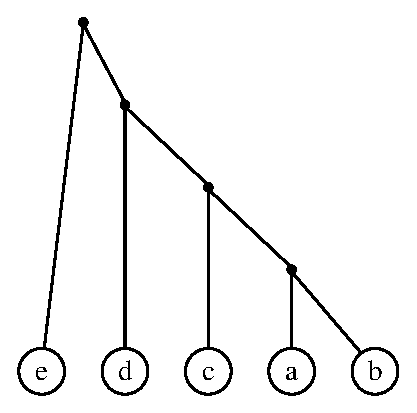
\includegraphics[width=3cm]{img/inp1.eps}
	\hspace{5mm}
	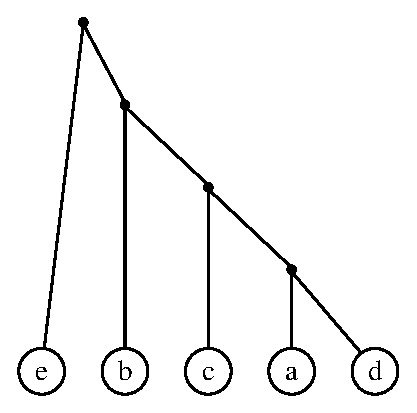
\includegraphics[width=3cm]{img/inp2.eps}
	\hspace{5mm}
	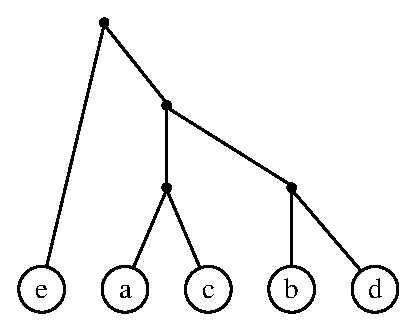
\includegraphics[width=3cm]{img/inp3.eps}
\end{figure}

Деревья над множеством таксонов \{a, b, c, d, e\}.

\end{frame}

\begin{frame}
\frametitle{Филогенетическое дерево}

\textbf{Проблемы?}

Гибридную модель эволюции невозможно представить в виде филогенетических деревьев.

\end{frame}

\begin{frame}
\frametitle{Гибридизационная сеть}

\begin{itemize}
	\item Мощнее чем филогенетическое дерево.
	\item Ретикулярные вершины - вершины с несколькими предками. Иллюстрируют гибридизационные события.
	\item Может иллюстрировать любую эволюционную историю.
\end{itemize}

\end{frame}

\begin{frame}
\frametitle{Гибридизационная сеть}

\centering

\begin{figure}[t]
	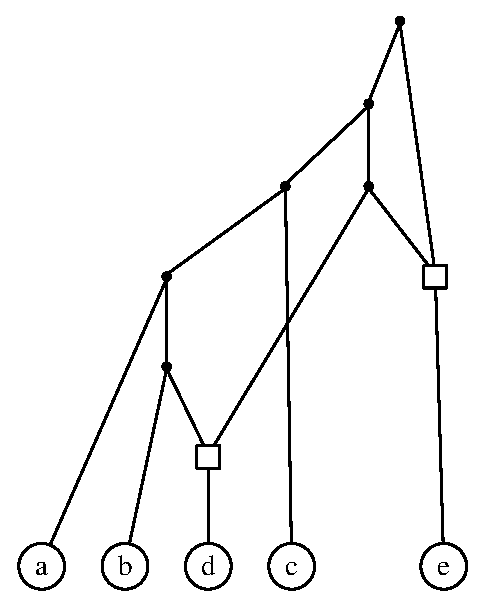
\includegraphics[width=2.8cm]{img/ans.eps}
	\hspace{1cm}
	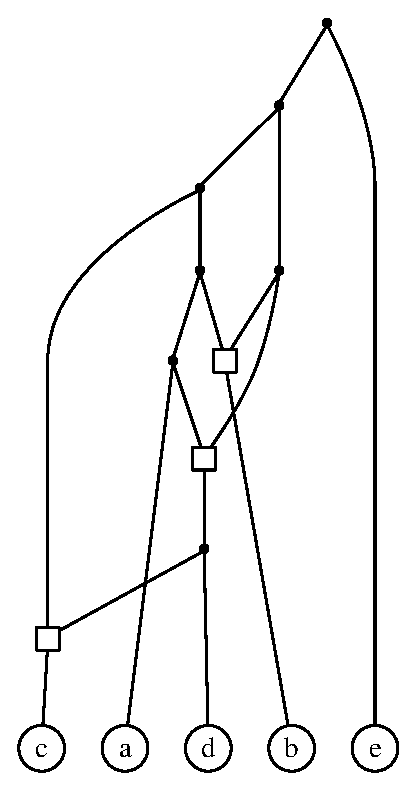
\includegraphics[width=2.8cm]{img/ans3.eps}
\end{figure}

Гибридизационные сети с двумя и тремя ретикулярными событиями соответственно.

\end{frame} 

\subsection{Постановка задачи}

\begin{frame}
\frametitle{Построение минимальной гибридизационной сети}

По набору филогенетических деревьев построить гибридизационную сеть с наименьшим количеством вершин, которая будет отображать одновременно все деревья.

\end{frame}

\begin{frame}
\frametitle{Построение минимальной гибридизационной сети}

\%Картинка с отображением дерева сетью\%

\end{frame}

\begin{frame}
\frametitle{Построение минимальной гибридизационной сети}

\textbf{Мотивация}: 
\begin{itemize}
	\item Маленькие гибридизационные сети проще анализировать, чем большие.
\end{itemize}


\textbf{Проблемы}:
\begin{itemize}
	\item NP-полная задача.
	\item Точные решения для деревьев больших размеров невозможно найти за разумное время.
\end{itemize}

\end{frame}

\subsection{Существующие решения}

\begin{frame}
\frametitle{Эвристические решения}

\begin{itemize}
	\item $\mathrm{PIRN_{CH}}$
	\item MURPAR
	\item CASS
\end{itemize}

\end{frame}

\begin{frame}
\frametitle{Точные решения}

\begin{itemize}
	\item $\mathrm{PIRN_C}$
\end{itemize}

\end{frame}

%Описание алгоритма
\section{Описание алгоритма}

\begin{frame}
\frametitle{Основная идея}

\begin{itemize}
	\item Переберем количество ретикулярных событий $h$.
	\item Построим формулу, которая выполнима тогда и только тогда, когда существует сеть с таким количеством ретикулярных событий.
	\item Найдем минимальное $h$, для которого формула выполнима.
\end{itemize}

\end{frame}


\begin{frame}
\frametitle{Построение формулы}

\begin{itemize}
	\item Структура сети.
	\item Связь исходных деревьев с сетью.
\end{itemize}

\end{frame}

\begin{frame}
\frametitle{Дополнения и оптимизации}

\begin{itemize}
	\item Выбор SAT-солвера.
	\item Быстрый поиск нижней и верхней границ $h$.
	\item Поиск всех возможных решений.
\end{itemize}

\end{frame}

%Тестирование и результаты
\section{Тестирование и результаты}

\subsection{Тестирование}

\begin{frame}
\frametitle{Методика тестирования}

\begin{itemize}
	\item Использовался набор реальных биологических данных, соответствующих злаковым травам.
	\item Для сравнения использовались алгоритмы $\mathrm{PIRN_C}$ и $\mathrm{PIRN_{CH}}$.
	\item Каждый алгоритм запускался с ограничением времени в 1000 секунд.
\end{itemize}

\end{frame}

\begin{frame}
\frametitle{Результаты точных алгоритмов}

\begin{table}
\centering
\begin{tabular}{l | l }
	& Решено тестов \\
	\hline
	PhyloSAT & 36 \\
	PIRN$\mathrm{_C}$ & 29 \\
\end{tabular}
\end{table}

\end{frame}

\begin{frame}
\frametitle{Результаты эвристических алгоритмов}

\begin{table}
\begin{tabular}{l | l }
	& Решено тестов \\
	\hline
	PhyloSAT & 48 \\
	PIRN$\mathrm{_{CH}}$ & 43 \\
\end{tabular}
\end{table}

На 12 тестах алгоритмы показали различающиеся результаты.

\begin{table}
\begin{tabular}{l | l | l}
	& Лучший результат & Лучшее время \\
	\hline
	PhyloSAT & 3 & 2 \\
	PIRN$\mathrm{_{CH}}$ & 2 & 5 \\
\end{tabular}
\end{table}

\end{frame}

\begin{frame}
\frametitle{Анализ нерешенных тестов}

\begin{table}
\begin{tabular}{l | l | l}
	Тест & Полученный ответ & Нижняя граница \\
	\hline
	RbclRpoc & \underline{7} & \underline{7} \\
	NdhfPhytIts & 13 & 11 \\
	NdhfPhytRpoc & 8 & 6 \\
	NdhfRbclRpoc & 12 & 10 \\
	NdhfWaxyIts & 8 & 7 \\
	PhytRbclIts & 9 & 7 \\
	PhytRpocIts & \underline{7} & \underline{7} \\
	RbclWaxyIts & \underline{6} & \underline{6} \\
	NdhfPhytRbclRpoc & 9 & 7 \\
	NdhfPhytRpocIts & 10 & 7 \\
	NdhfRbclWaxyIts & \underline{6} & \underline{6} \\	 
	PhytRbclRpocIts & 9 & 6 \\
\end{tabular}
\end{table}

\end{frame}

\subsection{Примеры полученных решений}

\begin{frame}

\%Картинка с двумя деревьями\%
	
\end{frame}

\begin{frame}

\%Картинка с решением для двух деревьев\%
	
\end{frame}

\begin{frame}

\%Картинка с тремя деревьями\%
	
\end{frame}

\begin{frame}

\%Картинка с решением для трех деревьев\%
	
\end{frame}

\subsection{Заключение}

\begin{frame}
\frametitle{Выводы}

\begin{itemize}
	\item PhyloSAT на данный момент является самым быстрым алгоритмом, гарантирующим нахождение точного решения
	\item Производительность PhyloSAT сравнима с производительностью эвристических алгоритмов
	\item Есть возможности для дальнейшего ускорения алгоритма
\end{itemize}

\end{frame}

\begin{frame}
\frametitle{Публикации}

Статья на конференцию AlCoB 2015.

Мехико, Мексика, Август 4--6, 2015.

\end{frame}

%Конец
\section{}

\begin{frame}
\frametitle{Спасибо за внимание!}

Вопросы?
\end{frame}


\end{document}